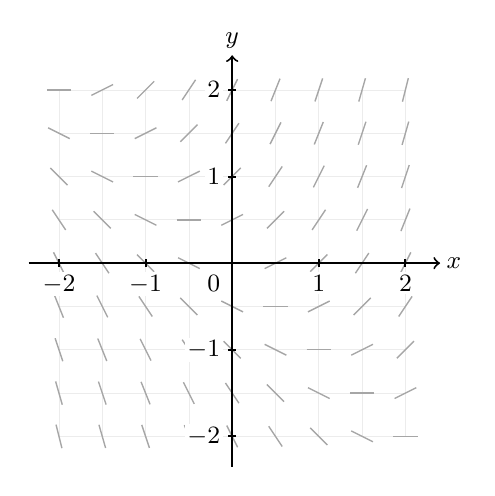
\begin{tikzpicture}[x=1.1cm,y=1.1cm,line width=.7pt,
  every node/.style={font=\small,inner sep=2pt}]
\draw[gray!15,line width=.25pt,step=.5] (-2,-2) grid (2,2);
\foreach \a in {-2,-1.5,...,2}{
  \foreach \b in {-2,-1.5,...,2}{
    \pgfmathsetmacro{\slope}{\a+\b}
    \pgfmathsetmacro{\run}{.14/sqrt(1+\slope*\slope)}
    \pgfmathsetmacro{\rise}{\slope*\run}
    \draw[gray!70,line width=.5pt]
      ({\a-\run},{\b-\rise})--({\a+\run},{\b+\rise});
  }
}
\draw[->] (-2.35,0)--(2.4,0);
\draw[->] (0,-2.35)--(0,2.4);
\node[right] at (2.4,0) {$x$};
\node[above] at (0,2.4) {$y$};
\foreach \a in {-2,-1,1,2}{
  \draw (\a,-.045)--(\a,.045);
  \node[below=3pt,fill=white,inner sep=1pt] at (\a,0) {$\a$};
  \draw (-.045,\a)--(.045,\a);
  \node[left=3pt,fill=white,inner sep=1pt] at (0,\a) {$\a$};
}
\node[below left=2pt] at (0,0) {$0$};
\end{tikzpicture}
